\section{Segnali Analogici}
    \subsection{Grandezze dei segnali Analogici}
    
        \subsubsection{Potenza istantanea}\label{Potenza istantanea}
                \begin{align}
                    P_{x} & \triangleq |x_{(t)}|^2 \nonumber \\   
                    Se\ x_{(t)} \in &\ \mathbb{R} \rightarrow P_{x} \triangleq x_{(t)}^2 \nonumber
                \end{align}
        \subsubsection{Energia}
            \[
                E_{x} \triangleq \int_{-\infty}^{\infty} P_{x}(t) \,dt = \int_{-\infty}^{\infty} |x_{(t)}|^2 \,dt    
            \]
            \[
                Energia:
                \begin{cases}
                    Energia\ finita \hspace{0.3cm}& (Segali\ fisici) \\
                    Energia\ infinita \hspace{0.3cm}& (Segali\ ideali)
                \end{cases}  
            \]
        \subsubsection{Potenza Media}\label{Potenza media}
            Definiamo il \index{Segnale Troncato}{\bf Segnale Troncato}:
                \[
                    x_{(t)} = X_{(t)} \triangleq 
                    \begin{cases}
                        x_{(t)} \hspace{1cm} -\frac{T}{2} \leq t \leq \frac{T}{2} \\
                        0 \hspace{2cm}altrove
                    \end{cases}
                    \]  
                    \begin{center}
                        \em T = Periodo di osservazione
                    \end{center}
                \begin{figure}[h]
                    \centering
                    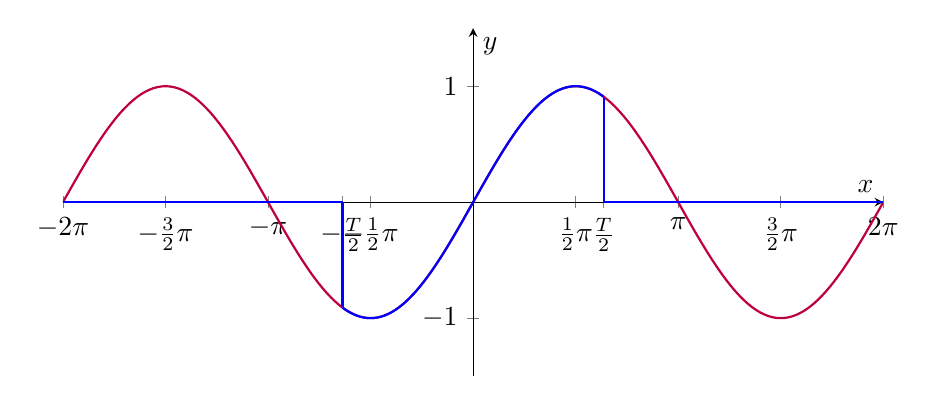
\begin{tikzpicture}
                        \begin{axis}[
                            domain=-2*pi:2*pi,
                            samples=200,
                            axis lines=middle,
                            xlabel=$x$,
                            ylabel=$y$,
                            ymin=-1.5,
                            ymax=1.5,
                            xtick={-2*pi, -3/2*pi, -pi, -1/2*pi,-2, 0, 2,1/2*pi, pi, 3/2*pi, 2*pi},
                            xticklabels={$-2\pi$, $-\frac{3}{2}\pi$, $-\pi$, $-\frac{1}{2}\pi$,$-\frac{T}{2}$, $0$, $\frac{T}{2}$, $\frac{1}{2}\pi$, $\pi$, $\frac{3}{2}\pi$, $2\pi$},
                            ytick={-1, 1},
                            yticklabels={$-1$, $1$},
                            width=12cm,
                            height=6cm
                        ]
                        \addplot [purple, thick] {sin(deg(x))};
                        \addplot [blue, thick, domain = -2:2] {sin(deg(x))};
                        \addplot [blue, thick, domain = 2:2*pi] {0};
                        \addplot [blue, thick, domain = -2*pi:-2] {0};
                        \addplot [const plot, thick,color=blue] coordinates {(-2,-0.9) (-2,0)};
                        \addplot [const plot, thick,color=blue] coordinates {(2,0.9) (2,0)};
                        \end{axis}
                    \end{tikzpicture}
                    \caption{Segnale troncato}
                    \label{fig:troncato}
                \end{figure}
            

            % NON CAPISCO COSA É POTENZA MEDIA E COSA SIA POTENZA ISTANTANEA CHE CAVOLO DI RELAZIONE
            % USO PER PASSARE DA PxT A Px  
            La potenza media é:
            \[
                P_{x_{T}} \triangleq \frac{E_{x_{T}}}{T}    
            \]
            \[
                E_{x_{T}} = \int_{-\frac{T}{2}}^{\frac{T}{2}}  |x_{(t)}|^2 \,dt  
            \]
            dalla quale possiamo ricavare se $T \rightarrow \infty \Rightarrow P_{x_{T}} = P_{x}$:
            \[
                P_{x} \triangleq \lim_{T\rightarrow\infty} \frac{E_{x_{T}}}{T} =\lim_{T\rightarrow\infty} \frac{1}{T} \int_{-\frac{T}{2}}^{\frac{T}{2}}  |x_{(t)}|^2 \,dt    
            \]  
            Possiamo ricavare delle propietá secondo energia e potenza:
            \begin{itemize}
                \item Se $x_{(t)}$ ha $E_x < \infty \Rightarrow P_x = 0$
                \item Se $x_{(t)}$ ha $P_x = k \neq 0 < \infty \Rightarrow E_x = \infty$
            \end{itemize}
        \subsubsection{Valore Efficace}\label{Valore Efficace}
                \[    
                    x_{eff} \triangleq \sqrt{P_{x}}
                \]
        
        \subsubsection{Valore Medio}\label{Valore medio}

                % TO DO: rivedi qui per evitare un page break
                    \[
                        x_{m} \triangleq \lim_{T\rightarrow\infty} \frac{1}{T} \int_{-\infty}^{\infty}  x_{(t)_T} \,dt = \lim_{T\rightarrow\infty} \frac{1}{T} \int_{-\frac{T}{2}}^{\frac{T}{2}}  x_{(t)} \,dt 
                    \]
                    \[
                        x_{(t)_T}\ =\ Segnale\ troncato
                    \]
                    
    \subsection{Analisi energetiche su segnali comuni}
        \subsubsection{Costante}
            $x_{(t)} = A\ \ \forall t$
            \begin{figure}[h]
                \centering
                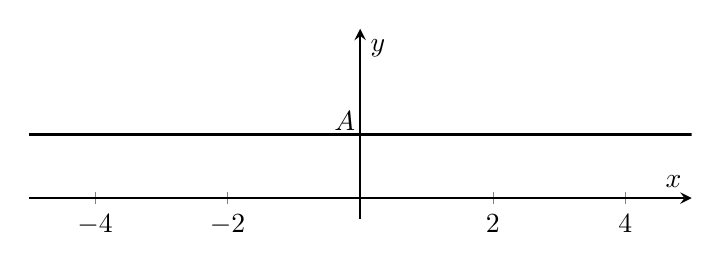
\begin{tikzpicture}
                    \begin{axis}[
                        xlabel=$x$,
                        ylabel=$y$,
                        xmin=-5,
                        xmax=5,
                        ymin=-0.5,
                        ymax=4,
                        ytick = {1.5},
                        yticklabels = {$A$},
                        yticklabel style = {yshift=5pt,xshift=4pt}, 
                        axis lines=middle,
                        thick,
                        domain=-5:5,
                        samples=100,
                        width=10cm,
                        height=4cm
                    ]
                    \addplot [const plot,black, thick] {1.5};
                    \end{axis}
                \end{tikzpicture}
                \caption{Segnale costante}
                \label{fig:segnale costante}
            \end{figure}
            \begin{itemize}
                \item {Energia:
                        \[
                            E_{x} = \int_{-\infty}^{\infty} P_{x}(t) \,dt = \int_{-\infty}^{\infty} |x_{(t)}|^2 \,dt = \int_{-\infty}^{\infty} A^2 \,dt = \infty 
                        \]
                }
                \item {Potenza Media:
                        \[
                            P_{x} = \lim_{T\rightarrow\infty} \frac{E_{x_{T}}}{T} = \lim_{T\rightarrow\infty} \frac{1}{T} \int_{-\frac{T}{2}}^{\frac{T}{2}}  |x_{(t)}|^2 \,dt = \lim_{T\rightarrow\infty} \frac{1}{T} \int_{-\frac{T}{2}}^{\frac{T}{2}} A^2 \,dt = A^2     
                        \]
                }
                \item {Valore Efficace:
                        \[
                            x_{eff} = \sqrt{P_{x}} = \sqrt{A^2} = |A|
                        \]
                }
                \item {Valore Medio:
                        \[
                            x_{m} = \lim_{T\rightarrow\infty} \frac{1}{T} \int_{-\frac{T}{2}}^{\frac{T}{2}}  x_{(t)} \,dt = \lim_{T\rightarrow\infty} \frac{1}{T} \int_{-\frac{T}{2}}^{\frac{T}{2}}  A \,dt = \lim_{T\rightarrow\infty} \frac{1}{T} AT = A 
                        \]
                }
            \end{itemize}
        
        \subsubsection{Cosinusoide}
            $x_{(t)} = A \cos(2 \pi f_0 t +\phi)$\\
            $A = Ampiezza,\  f_0= \frac{1}{T} = frequenza,\ \phi =fase$
            \begin{figure}[H]
                \centering
                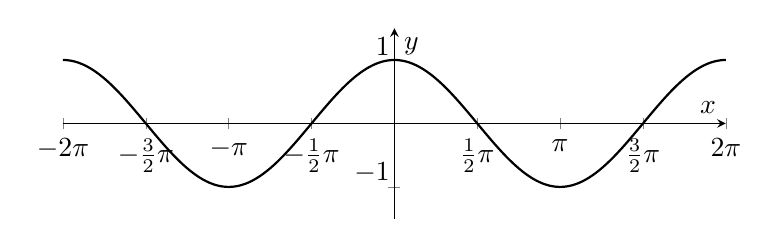
\begin{tikzpicture}
                    \begin{axis}[
                        domain=-2*pi:2*pi,
                        samples=200,
                        axis lines=middle,
                        xlabel=$x$,
                        ylabel=$y$,
                        ymin=-1.5,
                        ymax=1.5,
                        xtick={-2*pi, -3/2*pi, -pi, -1/2*pi, 0,1/2*pi, pi, 3/2*pi, 2*pi},
                        xticklabels={$-2\pi$, $-\frac{3}{2}\pi$, $-\pi$, $-\frac{1}{2}\pi$, $0$, $\frac{1}{2}\pi$, $\pi$, $\frac{3}{2}\pi$, $2\pi$},
                        ytick={-1, 1},
                        yticklabels={$-1$, $1$},
                        yticklabel style = {yshift=5pt,xshift=4pt}, 
                        width=10cm,
                        height=4cm
                    ]
                    \addplot [black, thick] {cos(deg(x))};
                    \end{axis}
                \end{tikzpicture}
                \caption{Segnale cosinusoidale ($\phi = 0$)}
                \label{fig:segnale sinusoidale}
            \end{figure}
            
            \begin{itemize}
                \item {Energia:
                    \[
                        E_{x} = \int_{-\infty}^{\infty} |x_{(t)}|^2 \ dt = \int_{-\infty}^{\infty} A^2 \cos^2(2\pi f_0 t + \phi) dt 
                    \]
                    Ricaviamo dalla $(1)$ \ref{Trigonometria} il $\sin^2(\alpha)$ e lo sostituiamo $(2.1)$ \ref{Trigonometria_Duplicazione} \\ $\cos(2\alpha) = \frac{1+ \cos^2(\alpha)}{2}$
                    \begin{align}
                            &= A^2  \int_{-\infty}^{\infty} \frac{1}{2} + \frac{\cos(4\pi f_0 t + 2\phi)}{2} dt \nonumber \\
                            &= A^2  \int_{-\infty}^{\infty} \frac{1}{2} dt + A^2 \int_{-\infty}^{\infty} \frac{\cos(4\pi f_0 t + 2\phi)}{2} dt \nonumber \\
                            &= \infty +\eval{\frac{A}{2} \frac{1}{4\pi f_0} \sin(4\pi f_0 t) }_{-\infty}^{\infty} = \infty \nonumber
                    \end{align}
                }
                \item {Potenza Media:
                    \begin{align}
                        P_{x} &=\lim_{T\rightarrow\infty}  \frac{1}{T} \int_{-\frac{T}{2}}^{\frac{T}{2}}  |x_{(t)}|^2 \,dt =\lim_{T\rightarrow\infty} \frac{1}{T} \int_{-\frac{T}{2}}^{\frac{T}{2}} A^2 \cos^2(2\pi f_0 t + \phi) dt \nonumber\\
                              &= \lim_{T\rightarrow\infty} \frac{1}{T} \frac{A}{2}T + \lim_{T\rightarrow\infty} \frac{A}{2}\int_{-\frac{T}{2}}^{\frac{T}{2}}\cos(4\pi f_0 t + 2\phi) dt  \nonumber\\
                              &= \frac{A}{2} + \lim_{T\rightarrow\infty} \eval{\frac{A}{2}\frac{1}{4\pi f_0}\sin(4\pi f_0 t + 2\phi)}_{\frac{T}{2}}^{-\frac{T}{2}} = \frac{A^2}{2} \nonumber
                    \end{align}
                }
                \item {Valore Efficace:
                    \[
                        x_{eff} = \sqrt{P_{x}} = \sqrt{\frac{A^2}{2}} =\frac{|A^2|}{\sqrt{2}} 
                    \]
                }
                \item {Valore Medio:
                    \begin{align}
                        x_{m} &= \lim_{T\rightarrow\infty} \frac{1}{T} \int_{-\frac{T}{2}}^{\frac{T}{2}}  x_{(t)} \,dt =\lim_{T\rightarrow\infty} \frac{1}{T} \int_{-\frac{T}{2}}^{\frac{T}{2}}\cos(2\pi f_0 t+\phi) dt \nonumber \\
                              &= \lim_{T\rightarrow\infty} \frac{1}{T}  \eval{\frac{A}{2}\frac{1}{2\pi f_0}\sin(2\pi f_0 t + \phi)}_{\frac{T}{2}}^{-\frac{T}{2}} = 0 \nonumber
                    \end{align}
                }
            \end{itemize}

            %Richimo per il label del formulario $(1)$ e $(2)$ \ref{Trigonometria} 
        \pagebreak
        \subsubsection{Gradino}
        $U_{(t)} = x_{(t)} = 
            \begin{cases}
                1 & t > 0 \\
                0 & t \leq 0  
            \end{cases}
        $
        \begin{figure}[H]
            \centering
            \begin{tikzpicture}
                \begin{axis}[
                    xlabel=$x$,
                    ylabel=$y$,
                    xmin=-5,
                    xmax=5,
                    ymin=-0.5,
                    ymax=4,
                    ytick = {1.5},
                    xtick = {},
                    xticklabels = {},
                    yticklabels = {$A$},
                    yticklabel style = {yshift=5pt,xshift=4pt}, 
                    axis lines=middle,
                    thick,
                    domain=-5:5,
                    samples=100,
                    width=10cm,
                    height=4cm
                ]
                \addplot [const plot,red, thick] coordinates{(0,1.5)(5,1.5)};
                \addplot [const plot,red, thick] coordinates{(0,0)(0,1.5)};
                \addplot [const plot,red, thick] coordinates{(-5,0)(0,0)};
                \end{axis}
            \end{tikzpicture}
            \caption{Segnale gradino}
            \label{fig:segnale gradino}
            
        \end{figure}        

        \begin{itemize}
            \item {Energia:
                \[
                    E_{x} = \int_{-\infty}^{\infty} |x_{(t)}|^2 \ dt = \int_{0}^{\infty} 1\ dt = \infty 
                \]
            }
            \item {Potenza Media:
                \[
                    P_{x} =\lim_{T\rightarrow\infty}  \frac{1}{T} \int_{-\frac{T}{2}}^{\frac{T}{2}}  |U_{(t)}|^2 \,dt =\lim_{T\rightarrow\infty} \frac{1}{T} \int_{0}^{\frac{T}{2}} 1\ dt = \lim_{T\rightarrow\infty} \frac{1}{T} \frac{T}{2} = \frac{1}{2}
                \]
            }
            \item {Valore Efficace:
                \[
                    x_{eff} = \sqrt{P_{x}} = \frac{1}{\sqrt{2}} 
                \]
            }
            \item {Valore Medio:
                    \[x_{m} = \lim_{T\rightarrow\infty} \frac{1}{T} \int_{-\frac{T}{2}}^{\frac{T}{2}}  x_{(t)} \,dt =\lim_{T\rightarrow\infty} \frac{1}{T} \int_{0}^{\frac{T}{2}} 1\ dt = \lim_{T\rightarrow\infty} \frac{1}{T} \frac{T}{2} = \frac{1}{2} \]
            }
        \end{itemize}
        
        \subsubsection{Rettangolo}
        $x_{(t)} = A\hspace{0.1cm}rect\left(\frac{t}{T}\right) =
            \begin{cases}
                A & -\frac{t}{T}\leq t\leq \frac{t}{T}\\
                0 & Altrove 
            \end{cases}
        $
        \begin{figure}[H]
            \centering
            \begin{tikzpicture}
                \begin{axis}[
                    xlabel=$x$,
                    ylabel=$y$,
                    xmin=-5,
                    xmax=5,
                    ymin=-0.5,
                    ymax=4,
                    ytick = {1.5},
                    xtick={-1.5, 0, 1.5},
                    xticklabels={$-\frac{T}{2}$, $0$, $\frac{T}{2}$},
                    yticklabels = {$A$},
                    yticklabel style = {yshift=5pt,xshift=4pt}, 
                    axis lines=middle,
                    thick,
                    domain=-5:5,
                    samples=100,
                    width=10cm,
                    height=4cm
                ]
                \addplot [const plot,red, thick] coordinates{(-1.5,1.5)(1.5,1.5)};
                \addplot [const plot,red, thick] coordinates{(-1.5,0)(-1.5,1.5)};
                \addplot [const plot,red, thick] coordinates{(1.5,0)(1.5,1.5)};
                \addplot [const plot,red, thick] coordinates{(5,0)(1.5,0)};
                \addplot [const plot,red, thick] coordinates{(-5,0)(-1.5,0)};
                \end{axis}
              \end{tikzpicture}
            \caption{Segnale rettangolo}
            \label{fig:segnale rettangolo}
        \end{figure}        
        \begin{itemize}
            \item {Energia:
                \[
                    E_{x} = \int_{-\infty}^{\infty} |x_{(t)}|^2 \ dt = \int_{-\frac{T}{2}}^{\frac{T}{2}} A^2 \hspace{0.1cm}rect^2\left(\frac{t}{T}\right)\ dt = A^2 \int_{-\frac{T}{2}}^{\frac{T}{2}}  1\ dt = A^2 T 
                \]
            }
            \item {Potenza Media:
                $T < T_0$ se non fosse cosí avrei una costante
                \begin{align}
                    P_{x} =\lim_{T\rightarrow\infty}  \frac{1}{T_0} \int_{-\frac{T_0}{2}}^{\frac{T_0}{2}}  |x_{(t)}|^2 \,dt & =\lim_{T\rightarrow\infty} \frac{1}{T_0}\int_{-\frac{T_0}{2}}^{\frac{T_0}{2}} A^2 \hspace{0.1cm}rect^2\left(\frac{t}{T}\right)\ dt \nonumber \\
                         & =\lim_{T\rightarrow\infty} \frac{1}{T_0} A^2 T = 0 \nonumber
                \end{align}
            }
            \item {Valore Efficace:
                \[
                    x_{eff} = \sqrt{P_{x}} = 0 
                \]
            }
            \item {Valore Medio:
                    \begin{align}
                        x_{m} = \lim_{T\rightarrow\infty} \frac{1}{T} \int_{-\frac{T}{2}}^{\frac{T}{2}}  x_{(t)} \,dt & = \lim_{T\rightarrow\infty} \frac{1}{T_0}\int_{-\frac{T_0}{2}}^{\frac{T_0}{2}} A\hspace{0.1cm}rect\left(\frac{t}{T}\right)\ dt \nonumber \\
                        & =\lim_{T\rightarrow\infty} \frac{1}{T_0} A T = 0 \nonumber
                    \end{align}
                    \begin{figure}[H]
                        \centering
                        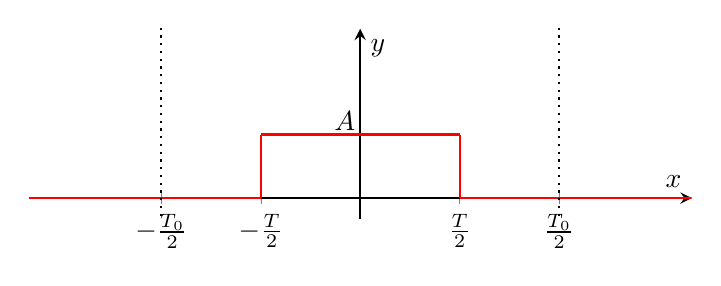
\begin{tikzpicture}
                            \begin{axis}[
                                xlabel=$x$,
                                ylabel=$y$,
                                xmin=-5,
                                xmax=5,
                                ymin=-0.5,
                                ymax=4,
                                ytick = {1.5},
                                xtick={-3,-1.5, 0, 1.5,3},
                                xticklabels={$-\frac{T_0}{2}$,$-\frac{T}{2}$, $0$, $\frac{T}{2}$, $\frac{T_0}{2}$},
                                yticklabels = {$A$},
                                yticklabel style = {yshift=5pt,xshift=4pt}, 
                                axis lines=middle,
                                thick,
                                domain=-5:5,
                                samples=100,
                                width=10cm,
                                height=4cm
                            ]
                            \addplot [const plot,red, thick] coordinates{(-1.5,1.5)(1.5,1.5)};
                            \addplot [const plot,red, thick] coordinates{(-1.5,0)(-1.5,1.5)};
                            \addplot [const plot,red, thick] coordinates{(1.5,0)(1.5,1.5)};
                            \addplot [const plot,red, thick] coordinates{(5,0)(1.5,0)};
                            \addplot [const plot,red, thick] coordinates{(-5,0)(-1.5,0)};
                            \addplot [const plot,dotted, black, thick] coordinates{(3,-5)(3,5)};
                            \addplot [const plot,dotted, black, thick] coordinates{(-3,-5)(-3,5)};
                            \end{axis}
                          \end{tikzpicture}
                        \caption{}
                        \label{fig:segnale rettangolo valore medio}
                    \end{figure}
            }
        \end{itemize}
        
        
        \subsubsection{Esponenziale unilatera}
        $x_{(t)} = e^{-t}U_{(t)}$
        \begin{figure}[H]
            \centering
            \begin{tikzpicture}
                \begin{axis}[
                    xlabel=$x$,
                    ylabel=$y$,
                    xmin=-5,
                    xmax=5,
                    ymin=-0.5,
                    ymax=4,
                    ytick = {1},
                    xtick={},
                    xticklabels={},
                    yticklabels = {$1$},
                    axis lines=middle,
                    thick,
                    domain=-5:5,
                    samples=100,
                    width=10cm,
                    height=4cm
                ]
                \addplot [domain= 0:5,samples = 100,red, thick] {exp(-x)};
                \end{axis}
              \end{tikzpicture}
            \caption{Segnale esponenziale unilatera}
            \label{fig:segnale esponenziale unilatera}
        \end{figure}        
        \begin{itemize}
            \item {Energia:
                \[
                    E_{x} = \int_{-\infty}^{\infty} |x_{(t)}|^2 \ dt = \int_{0}^{\infty} e^{-2t}\ dt = \eval*{-\frac{1}{2} e^{-2t}}_{0}^{\infty} = \frac{1}{2} 
                \]
            }
            \item {Potenza Media:
                \begin{align}
                    P_{x} & =\lim_{T\rightarrow\infty}  \frac{1}{T} \int_{-\frac{T}{2}}^{\frac{T}{2}}  |e^{-t}U_{(t)}|^2 \,dt =\lim_{T\rightarrow\infty} \frac{1}{T} \int_{0}^{\frac{T}{2}} e^{-2t}\ dt \nonumber \\
                          & = \lim_{T\rightarrow\infty} \frac{1}{T} \eval*{\left(-\frac{1}{2}\right) e^{-2t}}_{0}^{\frac{T}{2}} =\lim_{T\rightarrow\infty}-\frac{1}{2T} e^{-2\frac{T}{2}} + \lim_{T\rightarrow\infty} \frac{1}{2T} = 0 \nonumber 
                \end{align}
            }
            \item {Valore Efficace:
                \[
                    x_{eff} = \sqrt{P_{x}} = 0 
                \]
            }
            \item {Valore Medio:
                    \begin{align}
                        x_{m} & = \lim_{T\rightarrow\infty} \frac{1}{T} \int_{-\frac{T}{2}}^{\frac{T}{2}}  x_{(t)} \,dt =\lim_{T\rightarrow\infty} \frac{1}{T} \int_{-\frac{T}{2}}^{\frac{T}{2}} e^{-t}U_{(t)}\,dt = \lim_{T\rightarrow\infty} \frac{1}{T} \int_{0}^{\frac{T}{2}} e^{-t}\,dt \nonumber \\
                              & = \lim_{T\rightarrow\infty} \frac{1}{T} \eval*{(-1) e^{-t}}_{0}^{\frac{T}{2}} =  \lim_{T\rightarrow\infty}-\frac{1}{T} e^{-\frac{T}{2}} + \lim_{T\rightarrow\infty} \frac{1}{T} = 0 \nonumber
                    \end{align}
            }
        \end{itemize}
        
        \pagebreak
        \subsubsection{Esponenziale bilatera}
        $x_{(t)} = e^{-|t|}$
        \begin{figure}[H]
            \centering
            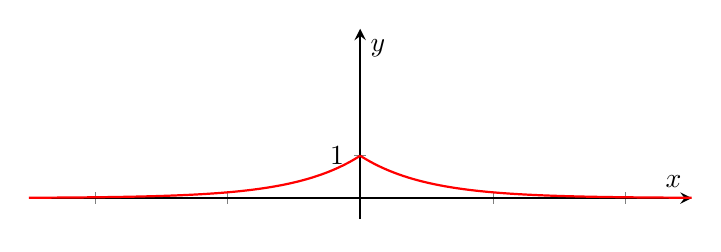
\begin{tikzpicture}
                \begin{axis}[
                    xlabel=$x$,
                    ylabel=$y$,
                    xmin=-5,
                    xmax=5,
                    ymin=-0.5,
                    ymax=4,
                    ytick = {1},
                    xtick={},
                    xticklabels={},
                    yticklabels = {$1$},
                    axis lines=middle,
                    thick,
                    domain=-5:5,
                    samples=100,
                    width=10cm,
                    height=4cm
                ]
                \addplot [domain= 0:5,samples = 100,red, thick] {exp(-x)};
                \addplot [domain= -5:0,samples = 100,red, thick] {exp(x)};
                \end{axis}
              \end{tikzpicture}
            \caption{Segnale esponenziale bilatera}
            \label{fig:segnale esponenziale bilatera}
        \end{figure}        
        \begin{itemize}
            \item {Energia:
                \[
                    E_{x} = \int_{-\infty}^{\infty} |x_{(t)}|^2 \ dt =2 \int_{0}^{\infty} e^{-2t}\ dt = \eval*{2 \left(-\frac{1}{2}\right) e^{-2t}}_{0}^{\infty} = 1 
                \]
            }
            \item {Potenza Media:
                \begin{align}
                    P_{x} & =\lim_{T\rightarrow\infty}  \frac{1}{T} \int_{-\frac{T}{2}}^{\frac{T}{2}}  |e^{-t}U_{(t)}|^2 \,dt =\lim_{T\rightarrow\infty} \frac{2}{T} \int_{0}^{\frac{T}{2}} e^{-2t}\ dt \nonumber \\
                          & = \lim_{T\rightarrow\infty} \frac{1}{T} \eval*{e^{-2t}}_{0}^{\frac{T}{2}} =\lim_{T\rightarrow\infty}-\frac{1}{T} e^{-2\frac{T}{2}} + \lim_{T\rightarrow\infty} \frac{1}{T} = 0 \nonumber 
                \end{align}
            }
            \item {Valore Efficace:
                \[
                    x_{eff} = \sqrt{P_{x}} = 0 
                \]
            }
            \item {Valore Medio:
                    \begin{align}
                        x_{m} & = \lim_{T\rightarrow\infty} \frac{1}{T} \int_{-\frac{T}{2}}^{\frac{T}{2}}  x_{(t)} \,dt =\lim_{T\rightarrow\infty} \frac{1}{T} \int_{-\frac{T}{2}}^{\frac{T}{2}} e^{-t}U_{(t)}\,dt = \lim_{T\rightarrow\infty} \frac{1}{T} 2\int_{0}^{\frac{T}{2}} e^{-t}\,dt \nonumber \\
                              & = \lim_{T\rightarrow\infty} \frac{1}{T} \eval*{(-2) e^{-t}}_{0}^{\frac{T}{2}} =  \lim_{T\rightarrow\infty}-\frac{2}{T} e^{-\frac{T}{2}} + \lim_{T\rightarrow\infty} \frac{2}{T} = 0 \nonumber
                    \end{align}
            }
        \end{itemize}        

        \subsubsection{segno $sgn(x_{(t)})$}
        $x_{(t)} = sgn(t) =
            \begin{cases}
                -1 & t < 0\\
                1  & t>0 
            \end{cases}
        $
        \begin{figure}[H]
            \centering
            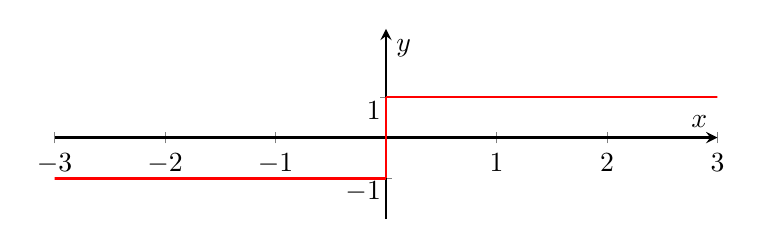
\begin{tikzpicture}
                \begin{axis}[
                    xlabel=$x$,
                    ylabel=$y$,
                    xmin=-3,
                    xmax=3,
                    ymin=-3,
                    ymax=4,
                    ytick={-1.5, 0, 1.5},
                    yticklabels = {$-1$,$0$,$1$},
                    yticklabel style = {yshift=-5pt,xshift=4pt}, 
                    axis lines=middle,
                    thick,
                    domain=-5:5,
                    samples=100,
                    width=10cm,
                    height=4cm
                ]
                \addplot [const plot,red, thick] coordinates{(0,1.5)(5,1.5)};
                \addplot [const plot,red, thick] coordinates{(0,-1.5)(0,1.5)};
                \addplot [const plot,red, thick] coordinates{(0,-1.5)(-5,-1.5)};
                \end{axis}
              \end{tikzpicture}
            \caption{Segnale sgn(x)}
            \label{fig:segnale sgn(x)}
        \end{figure}
        \begin{itemize}
            \item {Energia:
                \[
                    E_{x} = \int_{-\infty}^{\infty} |x_{(t)}|^2 \ dt = \int_{-\infty}^{\infty} sgn^2(t)\ dt = \int_{-\infty}^{\infty} 1\ dt =\infty 
                \]
            }
            \item {Potenza Media:
                \[
                    P_{x} =\lim_{T\rightarrow\infty}  \frac{1}{T} \int_{-\frac{T}{2}}^{\frac{T}{2}}  |x_{(t)}|^2 \,dt =\lim_{T\rightarrow\infty} \frac{1}{T} \int_{-\frac{T}{2}}^{\frac{T}{2}} sgn^2{t}\ dt = \lim_{T\rightarrow\infty} \frac{1}{T} T = 1
                \]
            }
            \item {Valore Efficace:
                \[
                    x_{eff} = \sqrt{P_{x}} = 1 
                \]
            }
            \item {Valore Medio:
                \begin{align}
                    x_{m} & = \lim_{T\rightarrow\infty} \frac{1}{T} \int_{-\frac{T}{2}}^{\frac{T}{2}}  x_{(t)} \,dt =\lim_{T\rightarrow\infty} \frac{1}{T} \int_{-\frac{T}{2}}^{\frac{T}{2}} sgn(t)\ dt \nonumber \\
                          & = \lim_{T\rightarrow\infty} \frac{1}{T} \left[\int_{-\frac{T}{2}}^{0}  1\,dt + \int_{0}^{\frac{T}{2}}  1\,dt\right] = \lim_{T\rightarrow\infty} \frac{1}{T} \left(-\frac{T}{2}+\frac{T}{2}\right) = 0 \nonumber
                \end{align}        
            }
        \end{itemize}
        
        \subsection{Segnal Periodici}
            Un segnale é periodico se: \\ 
            \[x_{(t)}=x_{(t-kT_0)}\hspace{0.5cm} k\in\mathbb{Z},\ t_0\in\mathbb{R}^+,\ T_0 = Periodo\ del\ segnale\]
            \begin{figure}[H]
                \centering
                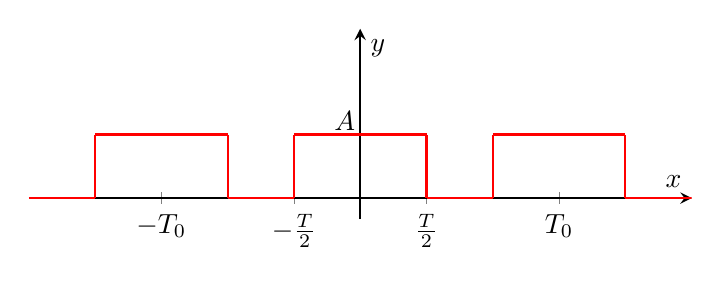
\begin{tikzpicture}
                    \begin{axis}[
                        xlabel=$x$,
                        ylabel=$y$,
                        xmin=-5,
                        xmax=5,
                        ymin=-0.5,
                        ymax=4,
                        ytick = {1.5},
                        xtick={-3,-1, 0, 1,3},
                        xticklabels={$-T_0$,$-\frac{T}{2}$, $0$, $\frac{T}{2}$,$T_0$},
                        yticklabels = {$A$},
                        yticklabel style = {yshift=5pt,xshift=4pt}, 
                        axis lines=middle,
                        thick,
                        domain=-5:5,
                        samples=100,
                        width=10cm,
                        height=4cm
                    ]
                    \addplot [const plot,red, thick] coordinates{(-1,1.5)(1,1.5)};
                    \addplot [const plot,red, thick] coordinates{(-1,0)(-1,1.5)};
                    \addplot [const plot,red, thick] coordinates{(1,0)(1,1.5)};
                    
                    \addplot [const plot,red, thick] coordinates{(-2,1.5)(-4,1.5)};
                    \addplot [const plot,red, thick] coordinates{(-2,0)(-2,1.5)};
                    \addplot [const plot,red, thick] coordinates{(-4,0)(-4,1.5)};
                    
                    \addplot [const plot,red, thick] coordinates{(2,1.5)(4,1.5)};
                    \addplot [const plot,red, thick] coordinates{(2,0)(2,1.5)};
                    \addplot [const plot,red, thick] coordinates{(4,0)(4,1.5)};
                    
                    \addplot [const plot,red, thick] coordinates{(2,0)(1,0)};
                    \addplot [const plot,red, thick] coordinates{(-2,0)(-1,0)};
                    \addplot [const plot,red, thick] coordinates{(-4,0)(-5,0)};
                    \addplot [const plot,red, thick] coordinates{(4,0)(5,0)};
                
                    \end{axis}
                  \end{tikzpicture}
                \caption{Segnale periodico}
                \label{fig:segnale periodico}
            \end{figure}     
            Si definiscono le seguenti grandezze: 
            \begin{itemize}
                \item {Energia di un segnale periodico
                    \begin{align}
                        E_{x} & = \int_{-\infty}^{\infty}  |x_{(t)}|^2 \,dt =\sum_{k=-\infty}^{\infty}\int_{-\frac{T_0}{2}+kT_0}^{\frac{T_0}{2}+kT_0} |x_{(t)}|^2 dt =\sum_{k=-\infty}^{\infty} X  \nonumber \\
                            & = \lim_{k\rightarrow\infty} kX= \infty \nonumber
                    \end{align}
                    Tutti i segnali periodici hanno quindi $E_x = \infty$   
                }
                \item {Potenza media di un segnale periodico
                    \begin{align}
                        P_{x} & = \lim_{T\rightarrow\infty} \frac{1}{T} \int_{-\frac{T}{2}}^{\frac{T}{2}}  |x_{(t)}|^2 \,dt\Rightarrow T = kT_0 \Rightarrow \lim_{k\rightarrow\infty} \frac{1}{kT_0} \int_{-\frac{kT_0}{2}}^{\frac{kT_0}{2}} |x_{(t)}|^2 dt \nonumber \\
                            & = \lim_{k\rightarrow\infty} \frac{1}{kT_0} k \int_{-\frac{T_0}{2}}^{\frac{T_0}{2}} |x_{(t)}|^2 dt  = \frac{1}{T_0} \int_{-\frac{T_0}{2}}^{\frac{T_0}{2}} |x_{(t)}|^2 dt \nonumber
                    \end{align}      
                    Posso calcolare la potenza di un singolo periodo:
                    \[
                        P_x = \frac{1}{T_0} \int_{-\frac{T_0}{2}}^{\frac{T_0}{2}} |x_{(t)}|^2 dt  
                    \]
                }
                \item {Valore medio di un segnale periodico
                    \[
                        x_m = \frac{1}{T_0} \int_{-\frac{T_0}{2}}^{\frac{T_0}{2}} x_{(t)} dt  
                    \]
                }
            \end{itemize}   